\chapter{Exoplaneter}
%
%
\begin{opgave}{Stjernernes spektre}{1}
Spektralklasser er et system, der opdeler stjerner efter deres temperatur. Figuren i dette link\footnote{\url{https://scienceruls.weebly.com/uploads/5/1/7/4/51741831/448172290.jpg}} viser forskellige spektraltyper, og visse absorptionslinjer er angivet. %?408
%\begin{figure*}[t]
%	\centering
%	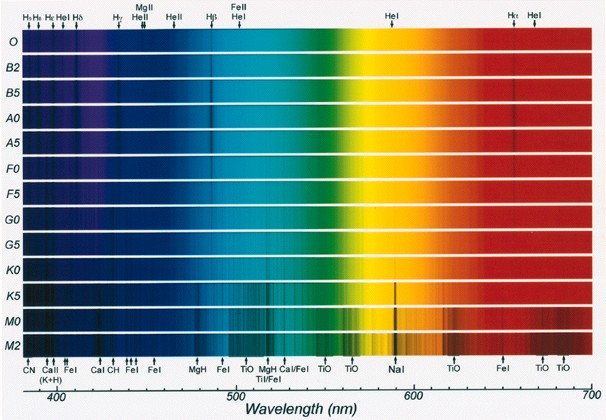
\includegraphics[width=\textwidth]{Astrofysik/billeder/stellar_abs.jpg}
%	\caption{Absorption for spektraltyper.}
%	\label{fig:stellar_abs}
%\end{figure*}
\opg Solen har spektralklasse G2V, men i dette tilfælde kan vi godt
tilnærme den til en G0-type. Hvad er nogle eksempler på stoffer,
som kan ses i dens atmosfære?
\opg Hvilke forskelle er der på stjernespektret fra en G0-type og de to M-typer?
\opg Stjerner af typerne M0 og M2 har en temperatur på $~\SI{3000}{\kelvin}$. Hvordan kan dette bruges til at forklare forskellen mellem M- og G-stjerner?
\end{opgave}
%
%
\begin{opgave}{Planetkandidater}{1}
Spektralklasserne er bestemt ud fra temperaturen som i tabel \ref{tab:spektral}.
\def\arraystretch{1.1}
\begin{table}[h!]
	\centering 
	\begin{tabular}{c|c}
		\textbf{Spektraltype} & \textbf{Temperatur} \\ \hline
		O             & \SI{40000}{\kelvin} \\
		B             & \SI{20000}{\kelvin} \\
		A             & \SI{9000}{\kelvin} \\
		F             & \SI{7000}{\kelvin} \\
		G             & \SI{5500}{\kelvin} \\
		K             & \SI{4500}{\kelvin} \\
		M             & \SI{3000}{\kelvin} \\
		L             & \SI{2000}{\kelvin} \\
		T             & \SI{1300}{\kelvin}          
	\end{tabular}
	\caption{Spektralklassifikation og temperaturer.}
	\label{tab:spektral}
\end{table}
\opg Hvilke stjernetyper er mest interessante at lede efter planter ved?
\opg Hvordan kan man identificere disse stjernetyper ud fra deres spektre?
\end{opgave}
%
%
\begin{opgave}{Stjernespektre og temperatur}{1}
For sortlegemer gælder Wiens forskydningslov
\begin{align*}
    \lambda_\text{max} = \frac{\SI{2.898e6}{\nano\metre\kelvin}}{T} \: ,
\end{align*}
hvor $T$ er sortlegemets temperatur, og $\lambda_\text{max}$ er bølgelængden for lyset med størst intensitet fra sortlegemet. 
\opg Ved hvilke bølgelængder skal en stjernes intensitetsmaksima ligge, for at være interessant at kigge efter planeter med liv omkring, under antagelse af at stjerner kan beskrives som sortlegemer?
\opg Kan dette lys ses med det menneskelige øje, og hvilken farve har det i så fald?
\end{opgave}
%
%
\begin{opgave}{Jævn cirkelbevægelse}{1}
Til at estimere massen af en planet fundet med radialhastighedsmetoden blev ligning \eqref{k-Pstar} i kompendiet benyttet. Den gælder under antagelse af jævn cirkelbevægelse.
\opg Beskriv i ord hvad jævn cirkelbevægelse vil sige.
\opg Vis at ligning \eqref{k-Pstar} gælder for jævn cirkelbevægelse.
\opg Benyt dette til at estimere Jordens fart i sin bane om Solen.
\end{opgave}
%
%
\begin{opgave}{Den Beboelige Zone}{1}
Jordens albedo er $A = 0,306$.
\opg Bestem den beboelige zone for en jordlignende planet: \\
a) \; I Solsystemet. \\
b) \; Om en anden stjerne, der er dobbelt så varm som Solen. \\
c) \; Om en tredje stjerne, hvis radius er 5 gange så stor som Solen.
\opg Kommenter resultatet for a). Giver det fysisk mening? Hvis ikke, hvad kan det skyldes?
\end{opgave}
%
%
\begin{opgave}{Gravitationslinser}{1}
I afsnit \ref{k-sec:GravLinse} i kompendiet om gravitationslinsemetoden blev det nævnt, at begivenheden skal observeres af flere forskellige målinger.
\opg Hvorfor er én måling ideelt set ikke nok?
\opg Hvorfor er det usandsynligt at observere samme planet med gravitationslinsemetoden mere end én gang?
\opg Hvordan medfører ovenstående, at planeten skal kunne ses i flere forskellige uafhængige målinger for at kunne kaldes en planet?
\end{opgave}
%
%
\begin{opgave}{Estimat af planetmasse}{2}
Vis med udgangspunkt i ligning \eqref{k-eq:K3Fancy} fra kompendiet, at ligning \eqref{k-eq:m_planet} i kompendiet gælder.
\end{opgave}
%
%
\begin{opgave}{Overfladetemperatur på planeter}{2}
Et sortlegeme er et legeme, som absorberer alt lys det bliver ramt af, og udsender det hele som varmestråling. Luminositeten fra et sfærisk sortlegeme givet som
\begin{align*}
    L = 4\pi R^2 \sigma T^4 \: ,
\end{align*}
hvor $R$ og $T$ er henholdsvis legemets radius og temperatur, og $\sigma$ er Boltzmanns konstant.
\opg Antag at stjerner opfører sig som sortlegemer, og vis at en planet med  radius $R_p$ i en afstand $D$ fra stjernen og med en albedo-værdi på $A$ vil absorbere energien
\begin{equation}
    L_\text{abs} = \frac{R_\star^2\sigma T_\star^4 \pi R_p^2}{D^2} \left(1 - A \right),
\end{equation}
hvor $R_\star$ og $T_\star$ er henholdsvis radius og temperatur af stjernen. \\
Hint: Man kan sige, at den del af planeten, der er vendt mod stjernen, udgør et areal givet ved $\pi R_m^2$. \\[2mm]
Antag at en planet også opfører sig som et sortlegeme, og at det er i termisk ligevægt.
\opg Hvad betyder det at planeten er i termisk ligevægt?
\opg Vis at temperaturen på overfladen af en planet, $T_p$, kan udtrykkes som
\begin{align*}
	T_p = T_\star \left( \frac{1-A}{4} \right)^{1/4} \left(\frac{R_\star}{D} \right)^{1/2} \, .
\end{align*}
\opg Antag at Saturns måne Mimas roterer hurtigt, samt at albedoen på overfladen af Mimas er $A_{Mimas} = 0,962$. Desuden oplyses det, at temperaturen på overfladen af Solen er $T_\odot = \SI{5778}{\kelvin}$, Solens radius er $R_\odot = \SI{6,955e5}{\kilo\metre}$, samt at middelafstanden mellem Mimas og Solen er $D_{\text{Mimas}} = \SI{1,43e9}{\kilo\metre}$. \\
Beregn ud fra oplysningerne en teoretisk temperatur på overfladen af Mimas. Gøre rede for dine antagelser. Cassini-rumsonden vurderede temperaturen på overfladen af Mimas til at være ca. \SI{65}{\kelvin}. Hvad kan forskellen mellem den teoretiske og den observede temperatur skyldes?
\end{opgave}
%
%
\def\arraystretch{1.3}
%
\begin{table}[h!]
    \centering
    \begin{tabular}{l|c}
        \textbf{Funktionel gruppe} & \textbf{Absorbtionslinje} \\ \hline
        OH (Alkohol) & \SIrange{2.74}{2.94}{\micro\metre} \\
        OH (Carboxylsyre) & \SIrange{3.24}{4,00}{\micro\metre} \\
        C=O (Keton) & \SIrange{5.62}{5.99}{\micro\metre} \\
    \end{tabular}
    \caption{Absorbtionslinjer for udvalgte organiske funktionelle grupper.}
    \label{tab:IR_linjer}
\end{table}
%
%
\begin{figure*}[h!]
    \centering
    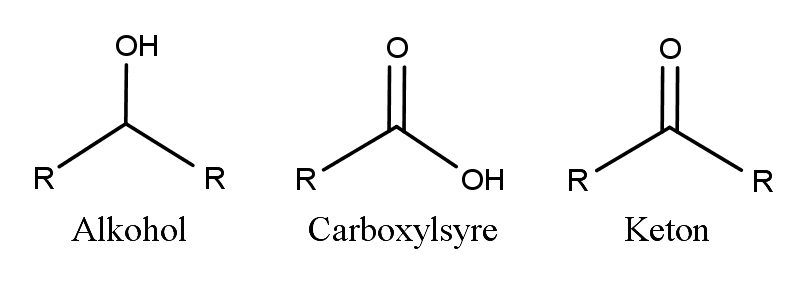
\includegraphics[width=.8\textwidth]{Astrofysik/billeder/grupper.png}
    \caption{Illustration af tre funktionelle, organiske grupper, tegnet i standardnotationen for organisk kemi. Det vil sige at hver streg repræsenterer en binding, hver knæk repræsenterer et C-atom og R står for en arbitrær gruppe kaldet et radikal. Yderligere er ikke-funktionelle H-atomer underforstået, hvorfor OH skrives, mens CH ikke skrives, idet H'et i CH ikke er kemisk aktivt.}
    \label{fig:grupper}
\end{figure*}   
%
%
\begin{opgave}{Spektre af planetatmosfærer}{2}
Ligesom individuelle atomer har specifikke spektre, så har molekyler det også, selvom dette er noget mere komplekst. Man bruger kemisk set typisk infrarød stråling, eftersom dette område giver de mest brugbare spektre. OH-gruppen i en alkohol ser anderledes ud en OH-gruppen i en carboxylsyre, fordi gruppens omgivelser er forskellige. Fælles for dem er dog, at de giver stærke brede absorptionslinjer, hvorfor de er relativt tydelige. Yderligere giver ketoner smalle, men stærke, absorptionslinjer. Tegninger af de forskellige funktionelle grupper ses i figur \ref{fig:grupper}, og deres absorptionslinjer ses i i tabel \ref{tab:IR_linjer}.
\opg Hvordan kan dette bruges i forbindelse med undersøgelsen af exoplaneter?
\opg Hvilke begrænsninger er der ved disse metoder? \\ \\ \\
\end{opgave}
%
%
\begin{opgave}{Atmosfærekrav}{3}
For at en planet kan have en stabil atmosfære, er den nød til at kunne holde simple molekyler fanget i dens tyngdefelt. Massen af $O_2$ er $m_{O_2} = \SI{5,31e-26}{\kilo\gram}$.
\opg Benyt Newtons gravitationslov og Newtons 2. lov til at bestemme tyngdeaccelerationen på en planets overflade.
\opg Er et legemes kinetiske energi præcis ligeså stor som det gravitationelle potentielle energi, vil den kunne undslippe det tyngdefelt det befinder sig i. Vis at denne hastighed, kaldet undvigelseshastigheden fra en planet, er givet som
\begin{align*}
	v_\mathrm{ecs}^2 = \frac{2M_pG}{R_p} \, .
\end{align*}
\opg Det oplyses nu fra kinetisk gasteori, at
\begin{align*}
	\frac{1}{2}mv_{av}^2 = \frac{3}{2}k_BT \, ,
\end{align*}
hvor $v_{av}$ er partiklerne i gassens gennemsnitlige fart, $m$ er partiklernes masse, $k_B$ er Boltzmanns konstant og $T$ er temperaturen i Kelvin. \\
Vis at
\begin{align*}
	\frac{M_p}{R_p} = \frac{3}{2}\frac{k_BT}{mG} \, ,
\end{align*}
hvis $v_\mathrm{ecs} = v_{av}$.
\opg Er $v_\mathrm{ecs} = v_{av}$ vil op mod halvdelen af molekyler med massen $m$ forsvinde væk fra planeten. Konkluder at for at en exoplanet kan fastholde $O_2$ i sin atmosfære, skal der om planeten gælde at
\begin{align} \label{eq:atm}
	\frac{M_p}{R_p} > \frac{3}{2}\frac{k_BT}{m_{O_2}G}
\end{align}
\opg Den gennemsnitlige temperatur på Jorden antages at være \SI{16}{\celsius}. Opfylder Jorden ligning \eqref{eq:atm}? \\
\end{opgave}
%
%
\begin{opgave}{Bose-Einsteinkondensat og laserkøling}{3}
For at lave Bose-Einstein kondensater i laboratoriet, skal man have nogle lette partikler, der køles ekstremt meget ned.\footnote{For den interesserede læser er et Bose-Einstein kondensat, at atomernes bølgefunktioner udvider sig, som temperaturen falder, indtil de tilsidst overlapper så meget, at du får en samlet bølgefunktion. De kan derfor betragtes som én stor partikel.} Mere præcist køles atomer (ofte alkalimetaller) ned til ~\SI{.1}{\micro\kelvin}, hvilket gøres ved først laserkøling og senere fordampningskøling. Laserkøling fungerer ved at udnytte at fotoner har impuls. Rammes et atom af en foton, der bevæger sig i modsat retning af atomet, exciteres det til et højere energiniveau, men dets fart falder også en smule for at bevare impulsen. Når atomet henfalder udsendes fotonen igen, og den accelereres en smule i en tilfældig retning. Sker dette mange gange, går disse små accelerationer ud med hinanden over tid, hvorved atomet bremses og atomskyen køles. Det virker dog kun, hvis man kan sikre sig, at atomer kun interagerer med fotoner, der bevæger sig i modsat retning af dem selv.
\opg Hvad er sammenhængen mellem en fotons energi og bølgelængde? \\
\opg Hvad sker der, hvis et atom rammes af en foton med en energi, der ikke svarer til en (tilladt) atomar overgang?\\ Hint: Tænk på atomet kvantemekanisk.\\ \\
Ved laserkølings sendes laserstråler ind fra seks retninger (positiv og negativ retning af hver af de kartesiske akser). Nu simplificeres systemet ved kun at kigge på systemet i én dimension. Betragt nu to ens atomer, der bevæger sig i hver sin retning. Fotonerne kommer fra en laser, der står stille i laboratoriet.
\opg Skiftes referencesystem til hvert atoms referenceramme, ser laseren ud til at bevæge sig. Hvorfor bevæger laseren sig ikke lige hurtigt i begge atomers referencesystem?
\opg Eftersom laseren bevæger sig Dopplerforskydes lyset. Hvad betyder forskellen i bevægelse for Dopplerforskydningen?
\opg Kan begge atomer exciteres af fotoner med samme bølgelængde?
\opg Hvordan kan dette bruges til at bremse atomerne selektivt?
\opg Er opgavetitlen clickbait?
\end{opgave}
%
%
\begin{opgave}{Masse af en planet}{2} \label{opg:MassePlanet}
Det kan vises at massen af en planet med radius $R$ og sfærisk symmetrisk densitet $\rho(r)$ (masse pr. volumen) er givet som
\begin{align} \label{eq:PlanetMasse}
    M = \int_0^R\rho(r)4\pi r^2\d r \: .
\end{align}
Det oplyses nu, at en planet har densitetsfunktionen
\begin{align*}
    \rho(r) = \begin{cases}
                \rho_0\left(1 - \frac{r}{R}\right)&, \quad r\leq R \\
                0 &, \quad r>R
                \end{cases}
\end{align*}
\opg Tegn $\rho(r)$.
\opg Hvad er planetens masse?
\end{opgave}
%
%
\begin{opgave}{Tyngdeacceleration indeni en planet}{3} \label{gPlanet}
Ikke nok med at en densitetsfunktion kan bruges til at bestemme hele massen af en planet, den kan også bruges til at bestemme tyngdeaccelerationen forskellige steder i planeten. Lad en planet med radius $R$ have densitetsfunktionen
\begin{align*}
    \rho(r) = \begin{cases}
               \dfrac{A}{r^2}\exp\left(\dfrac{r-R}{c}\right)&, \quad r\leq R \\[2mm]
                0 &, \quad r>R
                \end{cases}
\end{align*}
hvor $r$ er afstanden fra centrum, og $A,c$ er positive konstanter.
\opg Bestem enheden for $A$, for at $\rho(r)$ har den korrekte enhed.
\opg Forklar figur \ref{fig:PlanetDensitet}. \\ \\
Ud fra Newtons gravitationslov kan det vises at
\begin{align*}
    g(r) = G\frac{M(r)}{r^2} \: ,
\end{align*}
hvor $r$ er afstanden fra planetens centrum, $M$ den indesluttede masse, der er massen af den del af planten, der befinder sig i afstanden $r$ eller nærmere planetens centrum. Dette bygger også på antagelsen om sfærisk symmetri.
\opg Benyt ligning \eqref{eq:PlanetMasse} til at opskrive et udtryk for massen indenfor afstanden $r$.
\opg Bestemt tyngdeaccelerationen $g(r)$ udtrykt ved $r$ og eventuelle konstanter.
\end{opgave}
%%
%%
\begin{figure}[h!]
	\centering
	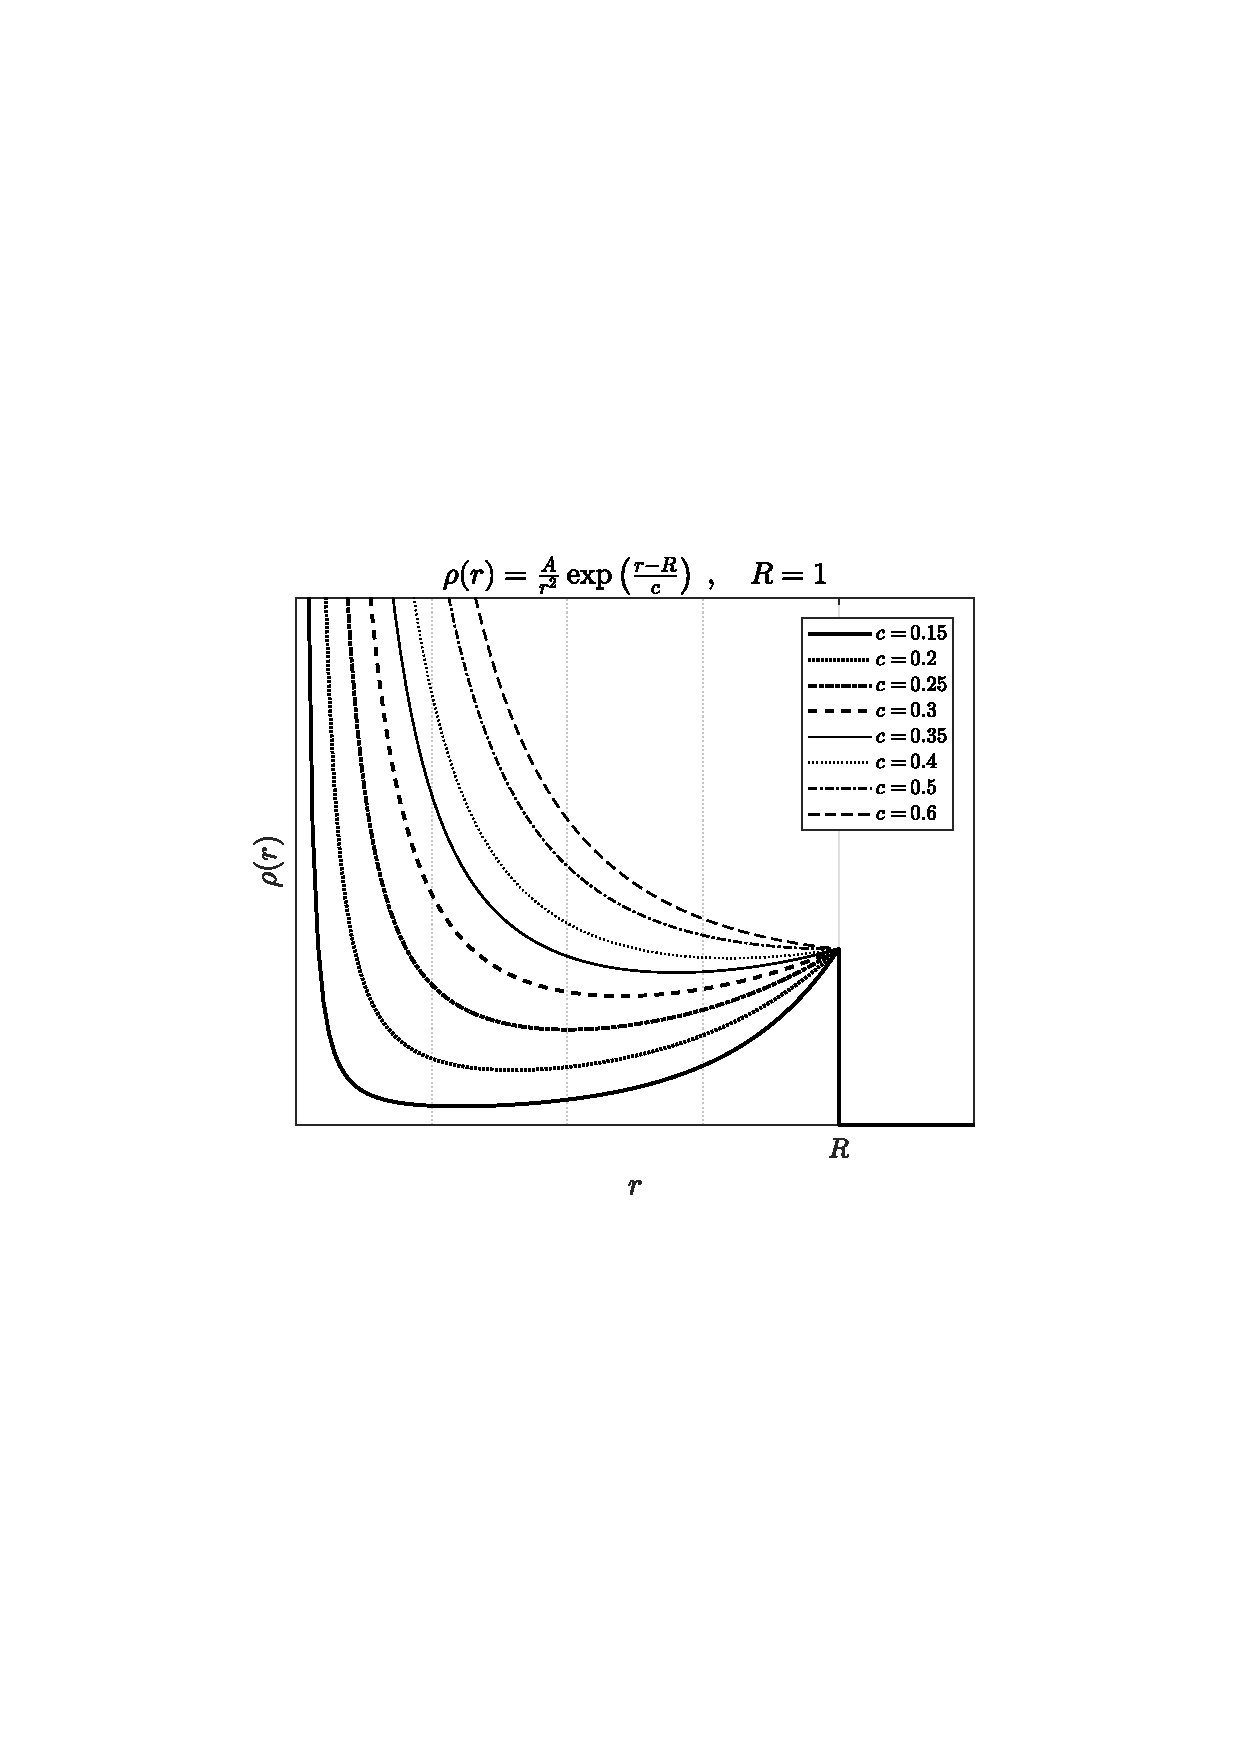
\includegraphics[trim=4.48cm 9.4cm 4.48cm 9.4cm,width=.9\columnwidth]{Astrofysik/billeder/g_i_planet.pdf}
	\caption{Plot af $g(r)$ for nogle forskellige værdier af $c$ og en fastholdt værdi af $R$.}
	\label{fig:PlanetDensitet}
\end{figure}